% Created 2018-10-04 Thu 19:58
% Intended LaTeX compiler: pdflatex
\documentclass[presentation]{beamer}
\usepackage[utf8]{inputenc}
\usepackage[T1]{fontenc}
\usepackage{graphicx}
\usepackage{grffile}
\usepackage{longtable}
\usepackage{wrapfig}
\usepackage{rotating}
\usepackage[normalem]{ulem}
\usepackage{amsmath}
\usepackage{textcomp}
\usepackage{amssymb}
\usepackage{capt-of}
\usepackage{natbib}
\usepackage[linktocpage,pdfstartview=FitH,colorlinks,
linkcolor=blue,anchorcolor=blue,
citecolor=blue,filecolor=blue,menucolor=blue,urlcolor=blue]{hyperref}
\setbeamertemplate{frame footer}{\insertshortauthor}
\setbeamerfont{page number in head/foot}{size=\tiny}
\setbeamercolor{footline}{fg=gray}
\author{Florian Hollenbach}
\usepackage[english]{isodate}
\usepackage{amsmath,amsthm,amssymb,amsfonts}
\usetheme{metropolis}
\usecolortheme{}
\usefonttheme{}
\useinnertheme{}
\useoutertheme{}
\author{Florian Hollenbach}
\date{\today}
\title{Political Science 209 - Fall 2018}
\subtitle{Prediction}

\hypersetup{
 pdfauthor={Florian Hollenbach},
 pdftitle={Political Science 209 - Fall 2018},
 pdfkeywords={},
 pdfsubject={},
 pdfcreator={Emacs 25.3.1 (Org mode 9.1.14)}, 
 pdflang={English}}
\begin{document}

\maketitle

\begin{frame}[label={sec:org70c5f35}]{In-class Exercise Measurement}
Carvalho, Leandro S., Meier, Stephen, and Wang, Stephanie W. (2016). ``Poverty and economic decision-making: Evidence from changes in financial resources at payday.'' American Economic Review, Vol. 106, No. 2, pp. 260-284.
\end{frame}


\begin{frame}[label={sec:orgb16ef53}]{In-class Exercise Measurement}
\emph{Do changes in one's financial circumstances affect one's decision-making process and cognitive capacity? In an experimental study, researchers randomly selected a group of US respondents to be surveyed before their payday and another group to be surveyed after their payday. Under this design, the respondents of the Before Payday group are more likely to be financially strained than those of the After Payday group. The researchers were interested in investigating whether or not changes in people's financial circumstances affect their decision making and cognitive performance. Other researchers have found that scarcity induce an additional mental load that impedes cognitive capacity.}
\end{frame}


\begin{frame}[label={sec:orgdb1859b}]{Poverty and economic decision-making}
In this study, the researchers administered a number of decision-making and cognitive performance tasks to the Before Payday and After Payday groups. We focus on the numerical stroop task, which measures cognitive control. In general, taking more time to complete this task indicates less cognitive control and reduced cognitive ability. They also measured the amount of cash the respondents have, the amount in their checking and saving accounts, and the amount of money spent.
\end{frame}

\begin{frame}[label={sec:org5915428}]{Poverty and economic decision-making}
Load the poverty.csv data set.
\end{frame}

\begin{frame}[label={sec:org55eda7f}]{Poverty and economic decision-making}
Variables:
\begin{itemize}
\item \emph{treatment}: Treatment conditions: Before Payday and After Payday

\item \emph{cash}: Amount of cash respondent has on hand

\item \emph{accts\_amt} Amount in checking and saving accounts

\item \emph{stroop\_time}: Log-transformed average response time for cognitive stroop test

\item \emph{income\_less20k}: Binary variable: 1 if respondent earns less than 20k a year and 0 otherwise
\end{itemize}

Look at a summary of the poverty data set to get a sense of what its variables looks like.
\end{frame}

\begin{frame}[label={sec:org569115c}]{Poverty and economic decision-making}
\alert{Question 1}

\begin{enumerate}
\item Use histograms to examine the univariate distributions of the two financial resources measures: cash and accts\_amt. What can we tell about these variables' distributions from looking at the histograms? Evaluate what the shape of these distributions could imply for the authors' experimental design.

\item Now, take the natural logarithm of these two variables and plot the histograms of these tranformed variables. How does the distribution look now? What are the advantages and disadvantages of transforming the data in this way?
\end{enumerate}

\alert{NOTE: Since the natural logarithm of 0 is undefined, researchers often add a small value (in this case, we will use \$1 so that \(\log 1 = 0\)) to the 0 values for the variables being transformed.}
\end{frame}

\begin{frame}[label={sec:orga1fa2f7}]{Poverty and economic decision-making}
\alert{Question 2a}

Now, let's examine the primary outcome of interest for this study-- the effect of a change in financial situation (in this case, getting paid on payday) on economic decision-making and cognitive performance. Begin by calculating the treatment effect for the stroop\_time variable (a log-transformed variable of the average response time for the stroop cognitive test), using first the mean and then the median. What does this tell you about differences in the outcome across the two experimental conditions?
\end{frame}


\begin{frame}[label={sec:org0efd352}]{Poverty and economic decision-making}
\alert{Question 2b}

Secondly, let's look at the relationship between finanical circumstances and the cognitive test variable. Produce two scatter plots side by side (hint: use the par(mfrow)) before your plot commands to place graphs side-by-side), one for each of the two experimental conditions, showing the bivariate relationship between your log-transformed cash variable and the amount of time it took subjects to complete the stroop cognitive test administered in the survey (stroop\_time). Place the stroop\_time variable on the y-axis. Be sure to title your graphs to differentiate between the Before Payday and After Payday conditions. Now do the same, for the log-transformed accts\_amt variable.
\end{frame}


\begin{frame}[label={sec:orgc8f5f1e}]{Poverty and economic decision-making}
\alert{Question 3}

Now, let's take a closer look at whether or not the Before Payday versus After Payday treatment created measurable differences in financial circumstances. What is the effect of payday on participants' financial resources? To help with interpretability, use the original variables cash and accts\_amt to calculate this effect. Calculate both the mean and median effect. Does the measure of central tendency you use affect your perception of the effect?
\end{frame}


\begin{frame}[label={sec:org1be4f71}]{Poverty and economic decision-making}
\alert{Question 4}

Compare the distributions of the Before Payday and After Payday groups for the log-transformed cash and accts\_amt variables. Use quantile-quantile plots to do this comparison, and add a 45-degree line in a color of your choice (not black). Briefly interpret your results and their implications for the authors' argument that their study generated variation in financial resources before and after payday. When appropriate, state which ranges of the outcome variables you would focus on when comparing decision-making and cognitive capacity across these two treatment conditions.
\end{frame}


\begin{frame}[shrink=15,label={sec:org9177564}]{Poverty and economic decision-making}
\alert{Question 5}

In class, we covered the difference-in-difference design for comparing average treatment effects across treatment and control groups. This design can also be used to compare average treatment effects across different ranges of a pre-treatment variable- a variable that asks about people's circumstances before the treatment and thus could not be affected by the treatment. This is known as heterogeneous treatment effects -- the idea that the treatment may have differential effects for different subpopulations. Let's look at the pre-treatment variable income\_less20k. Calculate the treatment effect of Payday on amount in checking and savings accounts separately for respondents earning more than 20,000 dollars a year and those earning less than 20,000 dollars. Use the original accts\_amt variable for this calculation. Then take the difference between the effects you calculate. What does this comparison tell you about how payday affects the amount that people have in their accounts? Are you convinced by the authors' main finding from Question 2 in light of your investigation of their success in manipulating cash and account balances before and after payday?
\end{frame}


\begin{frame}[label={sec:orgc12d68b}]{Prediction}
\begin{center}

\includegraphics[width=8cm]{/Users/florianhollenbach/Documents/GitHub/Polisci209_2018/slides/week6/paul.png}
\end{center}
\end{frame}


\begin{frame}[label={sec:org00a77b9}]{Prediction}
\begin{itemize}
\item One important task of (social) scientists can be \emph{prediction}
\item Forecasting future events, e.g., conflict, unrest, elections
\item Causal inference, also involves prediction, of what?
\end{itemize}
\pause
\begin{itemize}
\item To estimate the causal effect we are essentially predicting the \emph{counterfactual}
\end{itemize}
\end{frame}


\begin{frame}[label={sec:org34f5b72}]{Prediction}
\begin{center}
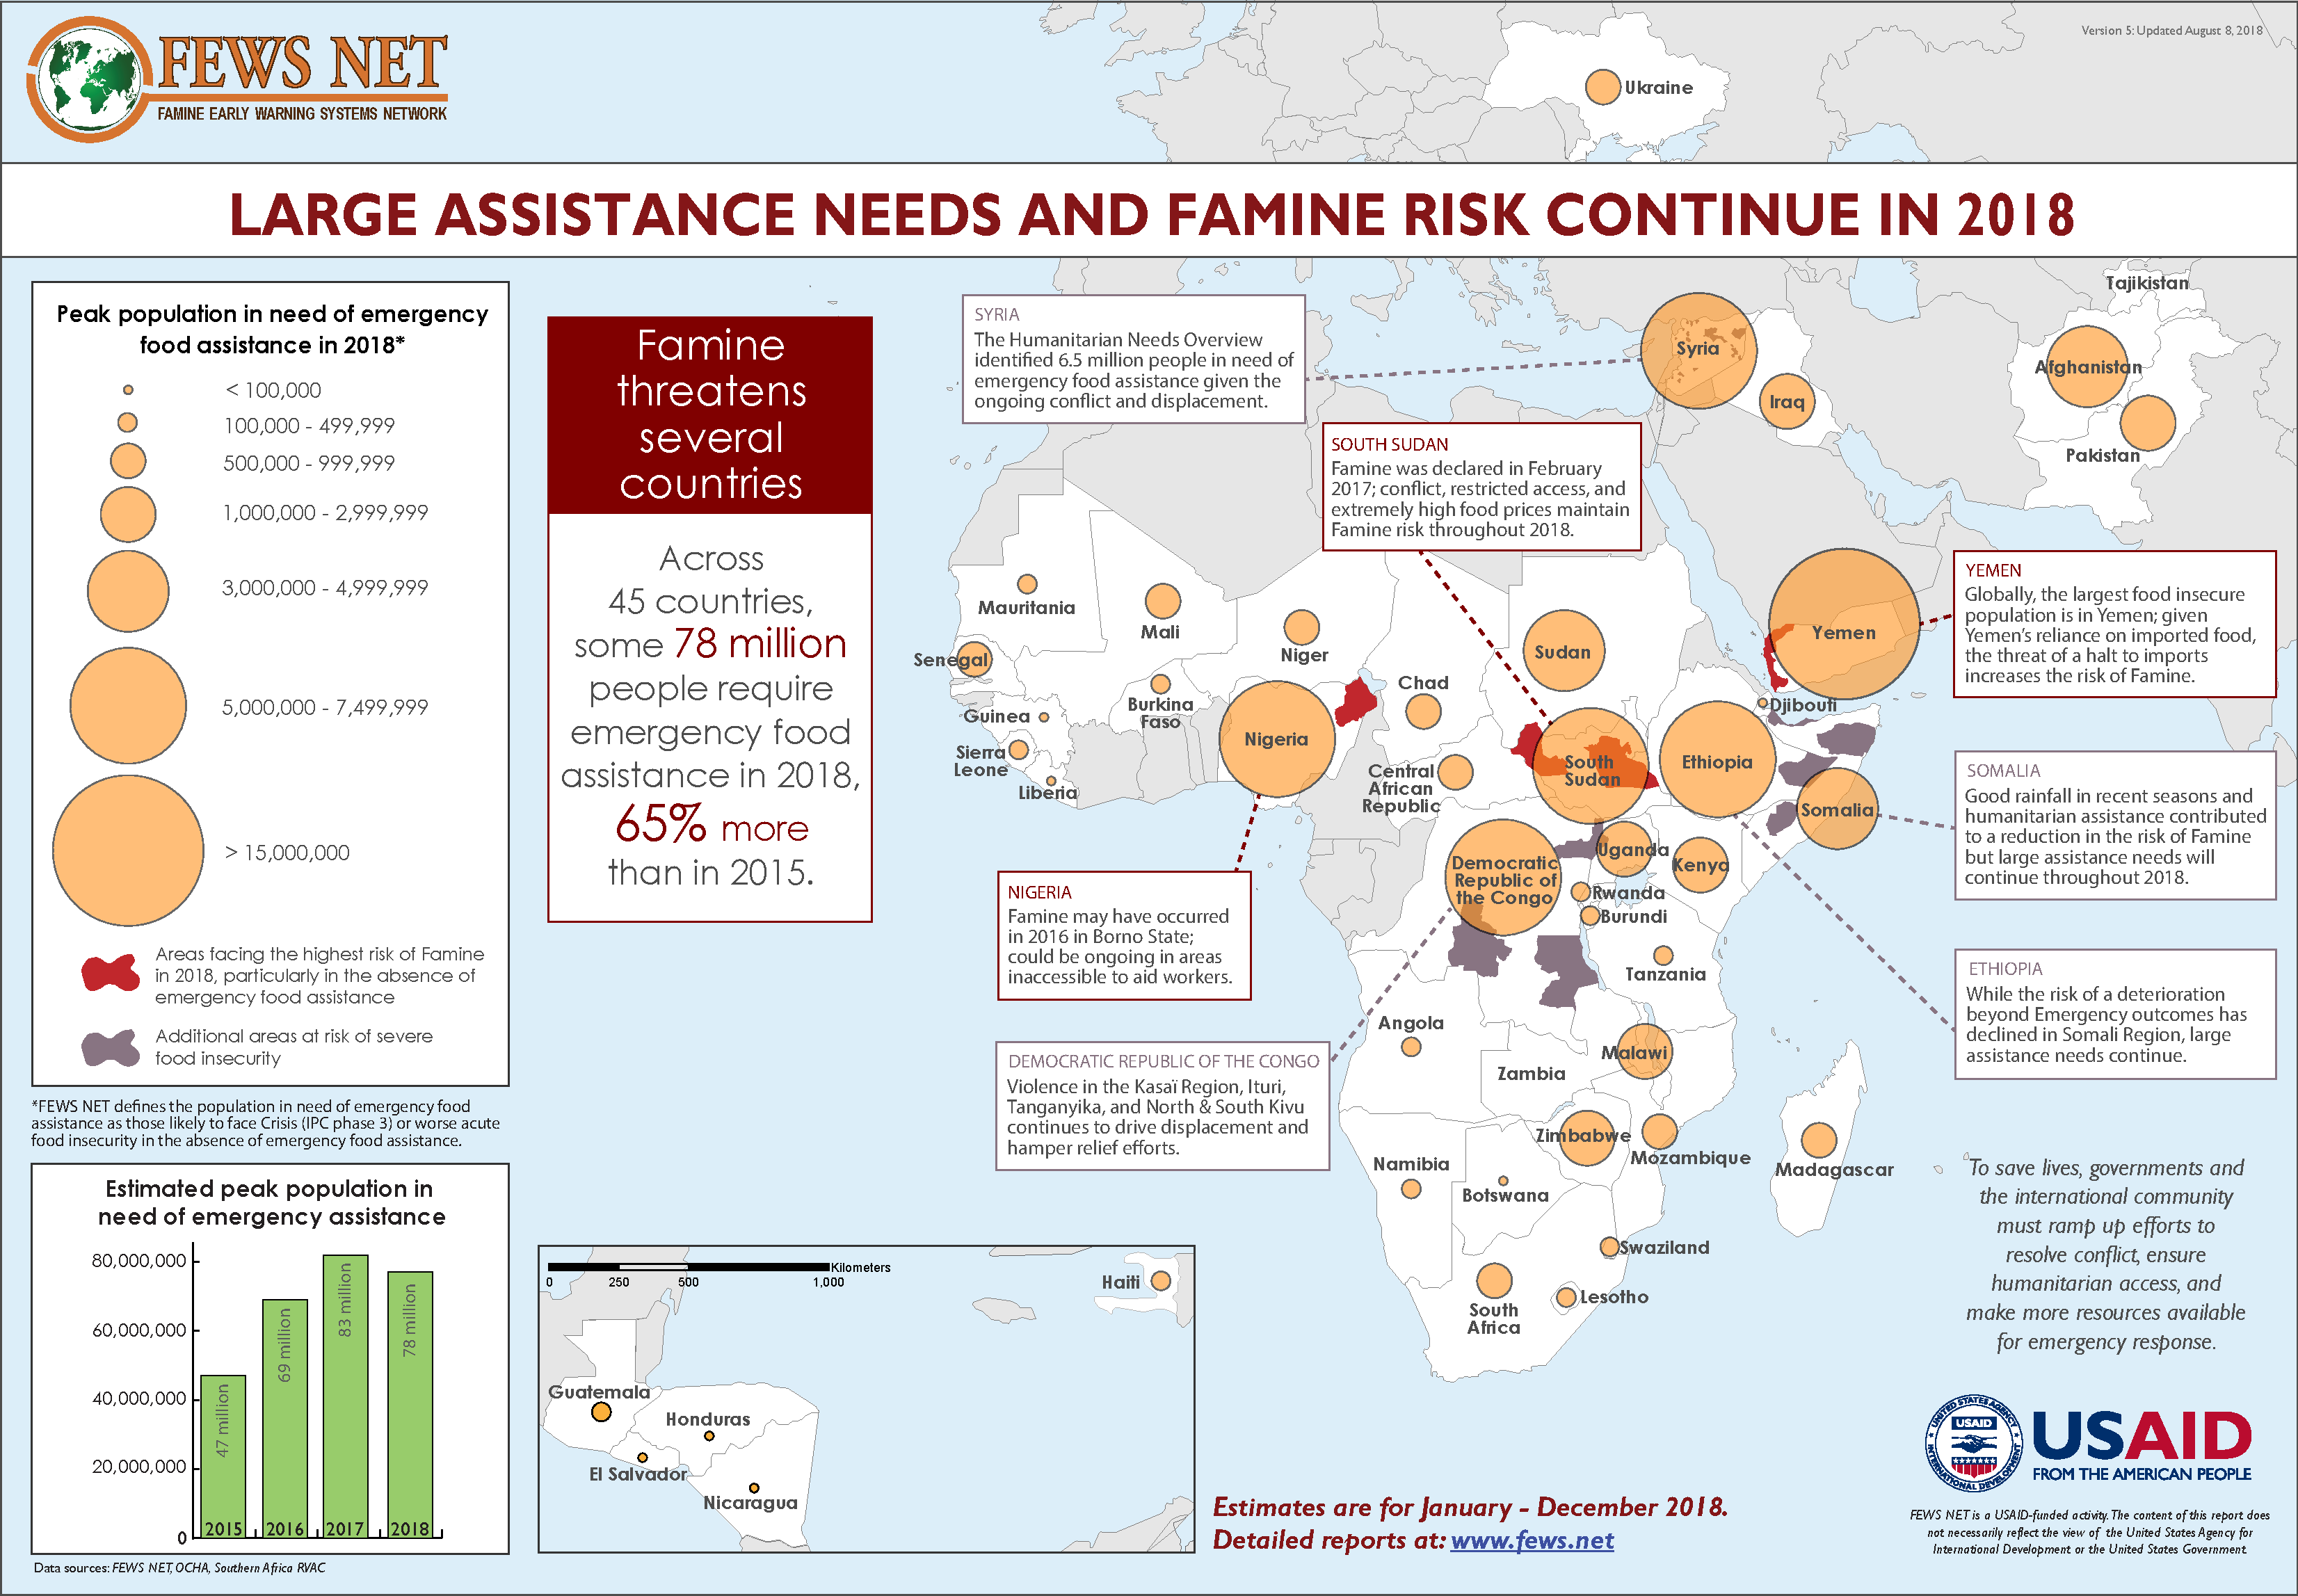
\includegraphics[width=8cm]{/Users/florianhollenbach/Documents/GitHub/Polisci209_2018/slides/week6/famine.pdf}
\end{center}
\end{frame}



\begin{frame}[label={sec:org248589f}]{Prediction}
\begin{center}
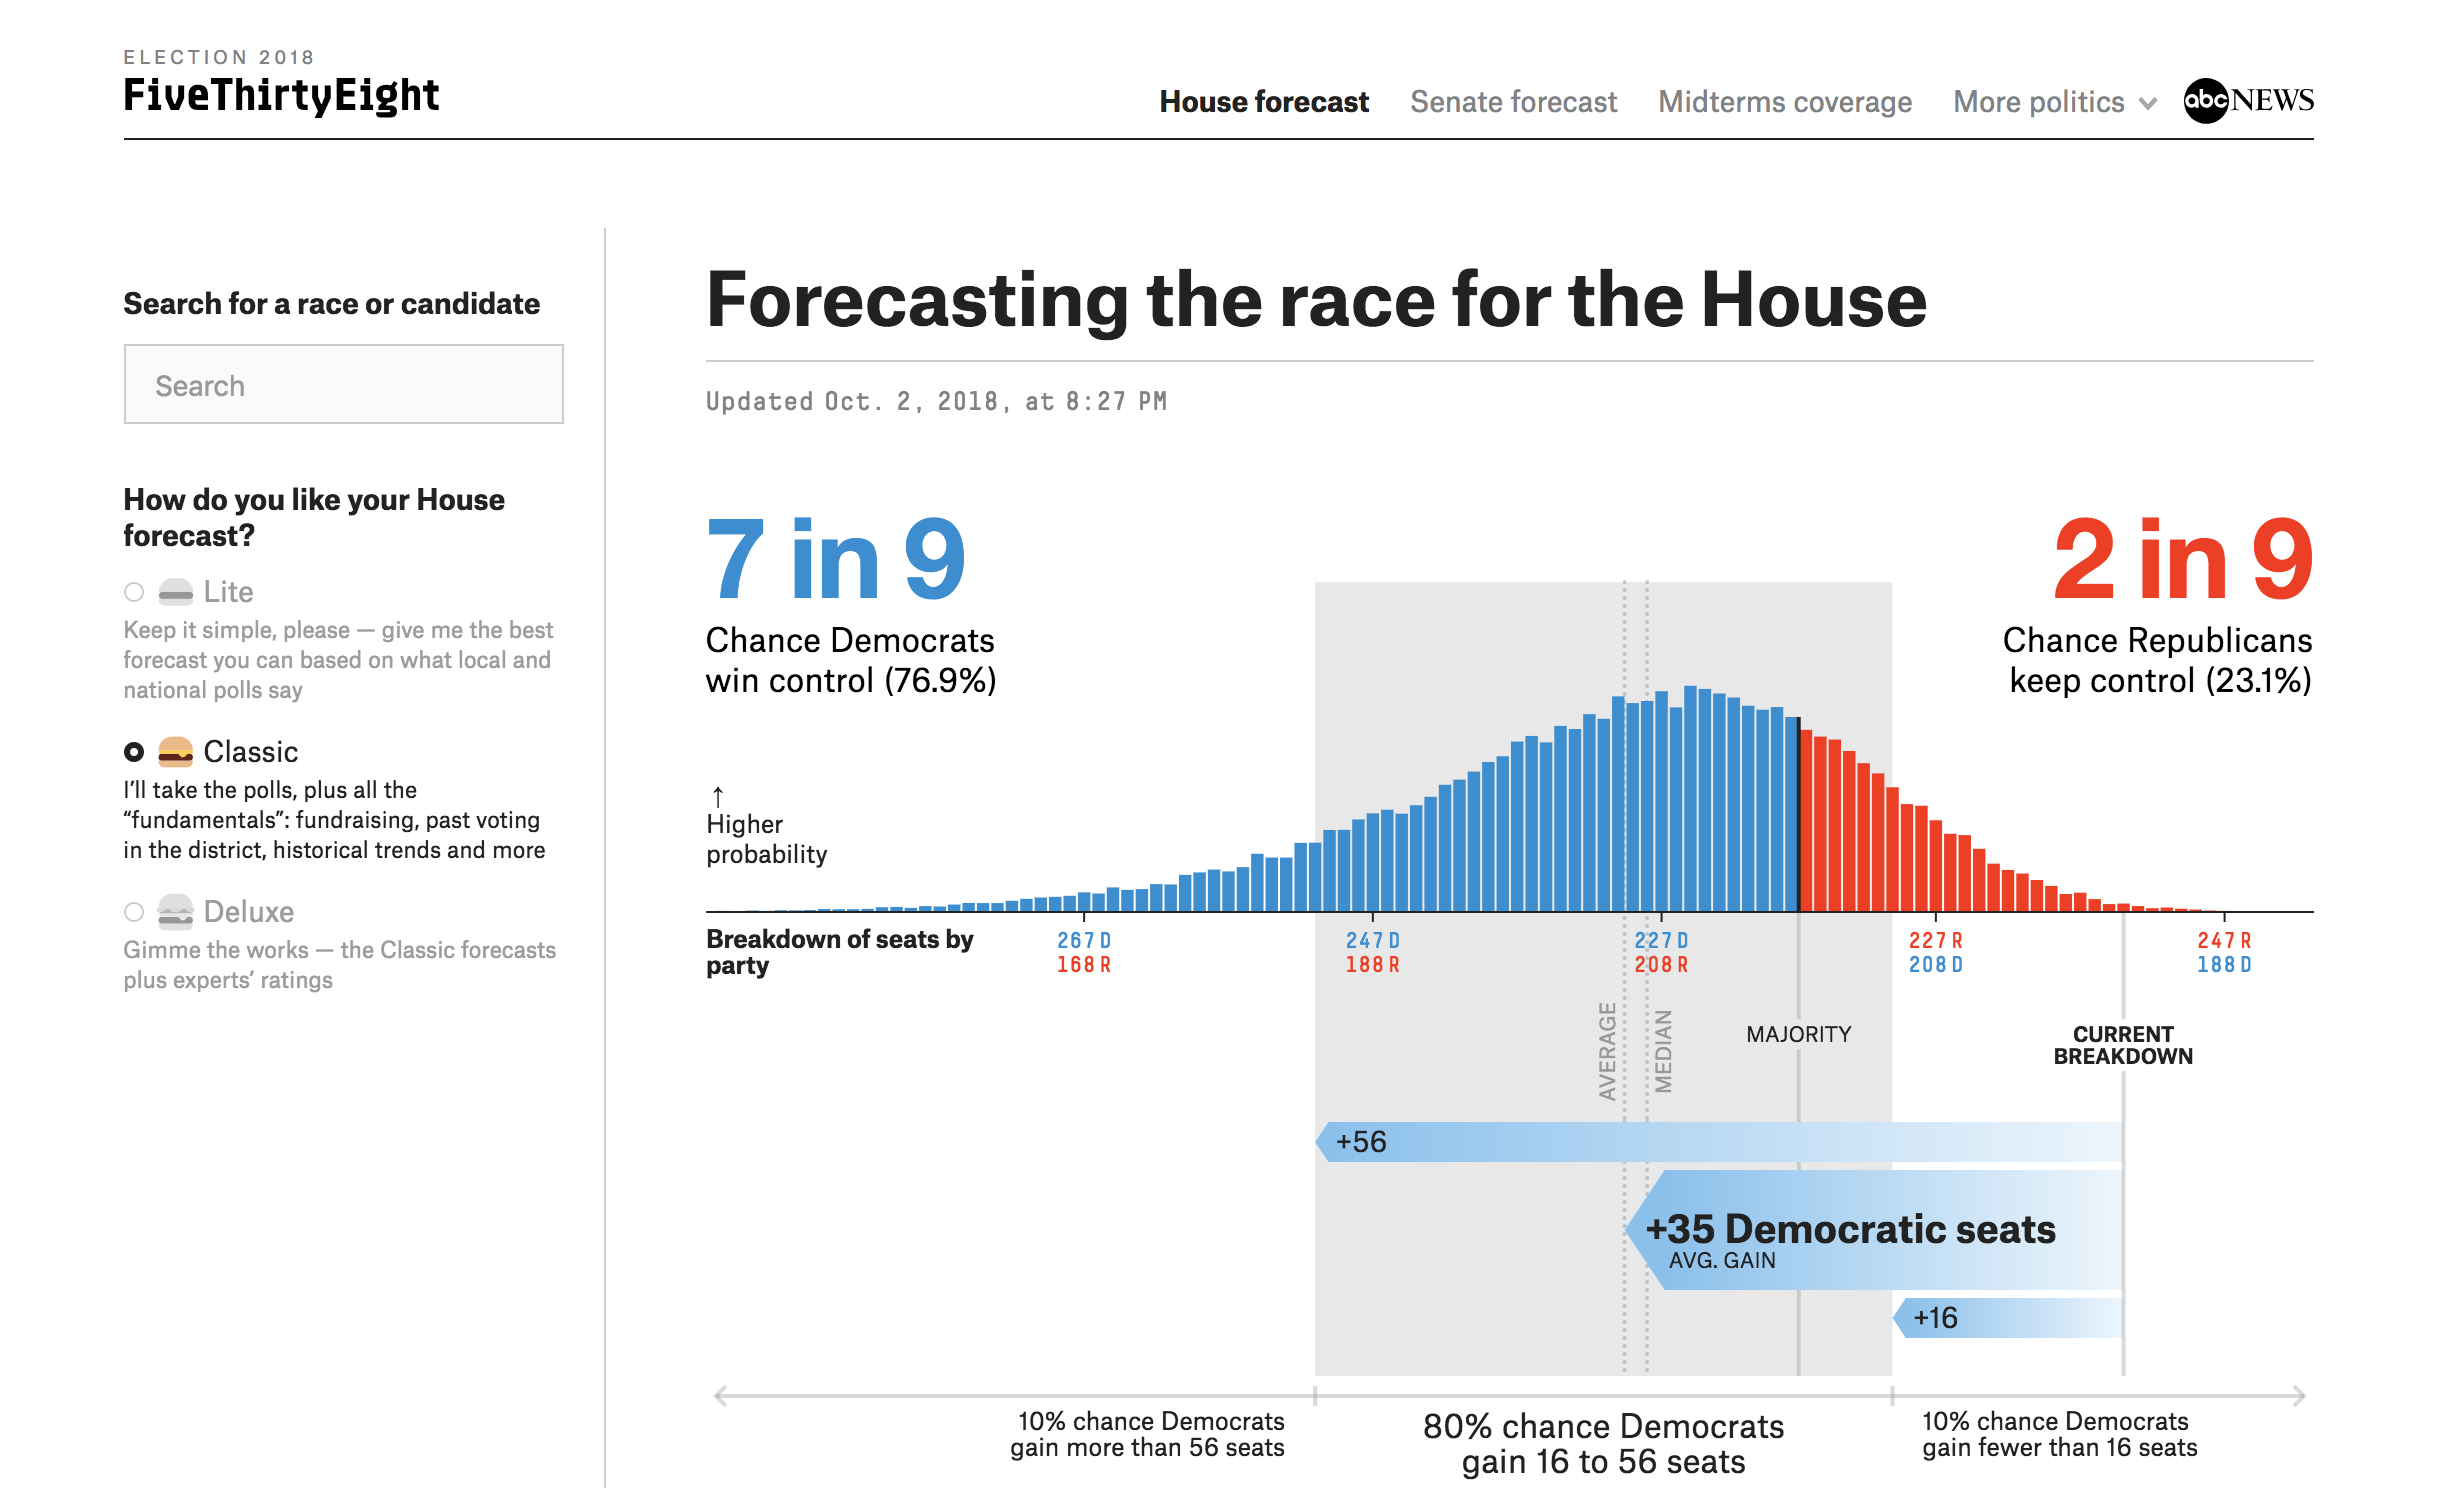
\includegraphics[width=8cm]{/Users/florianhollenbach/Documents/GitHub/Polisci209_2018/slides/week6/five38.png}
\end{center}
\end{frame}





\begin{frame}[label={sec:org012ddb7}]{Prediction}
\begin{itemize}
\item Elections can be predicted using fundamentals
\end{itemize}

\pause

\begin{itemize}
\item Or we can use polls to predict results
\end{itemize}
\end{frame}


\begin{frame}[label={sec:org0cf4a8b}]{Prediction with polls}
\begin{itemize}
\item We will use a nice \emph{R} package called \emph{pollstR}, which
scrapes the data from Huffington Post:
\end{itemize}

\begin{center}
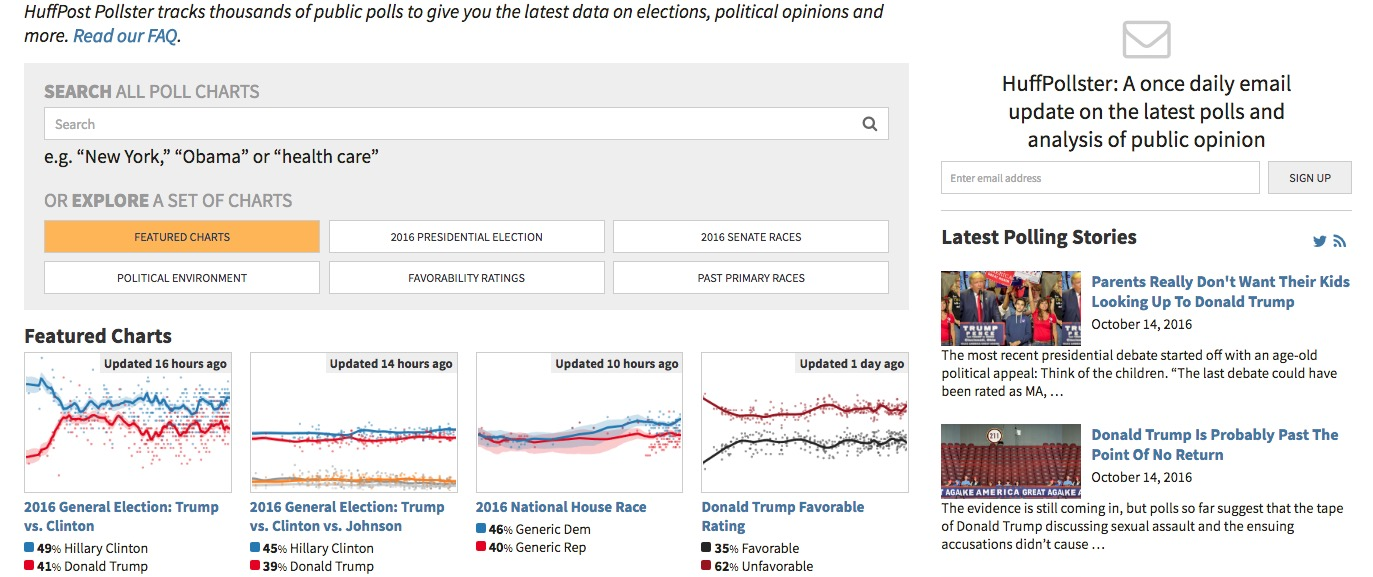
\includegraphics[width=8cm]{/Users/florianhollenbach/Documents/GitHub/Polisci209_2018/slides/week6/pollsterWebPage.png}
\end{center}
\end{frame}

\begin{frame}[fragile,shrink=15,label={sec:org98e4a6f}]{Prediction with polls}
 \begin{verbatim}
library(pollstR)
chart_name <- "2016-general-election-trump-vs-clinton"
polls2016 <- pollster_charts_polls(chart_name)[["content"]]
\end{verbatim}
\end{frame}


\begin{frame}[fragile,label={sec:org72db9bc}]{Prediction with polls}
 \begin{itemize}
\item Let's calculate a variable that is \emph{days until the election}
\end{itemize}

\begin{verbatim}
class(polls2016$end_date)
polls2016$DaysToElection <-
    as.Date("2016-11-8") - polls2016$end_date
\end{verbatim}
\end{frame}

\begin{frame}[fragile,shrink=25,label={sec:org09615ee}]{Prediction with polls}
 We could make a very simple plot of all the polls over time
\begin{verbatim}
plot(polls2016$DaysToElection, polls2016$Clinton,
     xlab = "Days to the Election", ylab = "Support",
     xlim = c(550, 0), ylim = c(25, 65), pch = 19,
     col = "blue")
points(polls2016$DaysToElection, polls2016$Trump,
       pch = 20, col = "red")
\end{verbatim}
\end{frame}



\begin{frame}[label={sec:orgadaef55}]{Prediction with polls}
\begin{center}
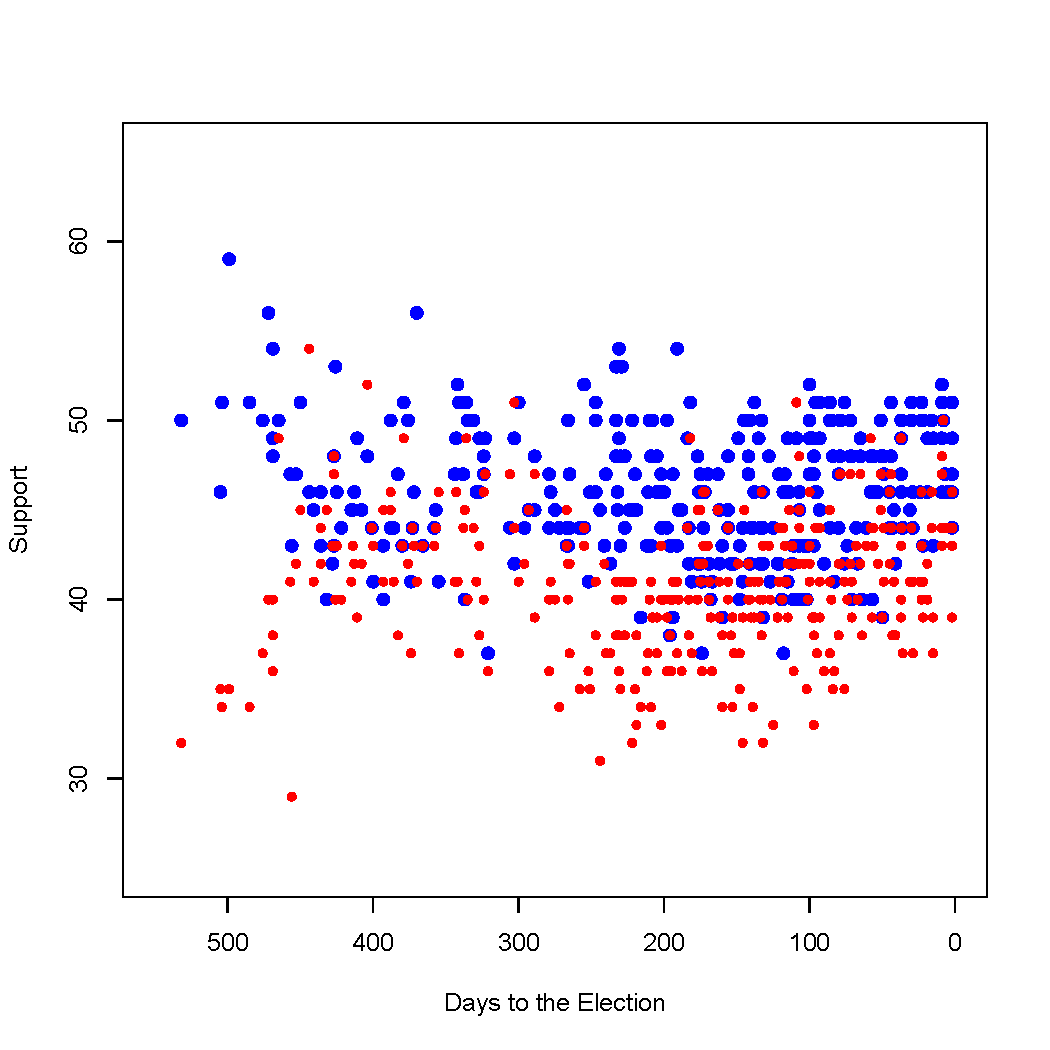
\includegraphics[width=5cm]{/Users/florianhollenbach/Documents/GitHub/Polisci209_2018/slides/week6/simplePolls.pdf}
\end{center}

\alert{But that looks kind of dumb}

\pause
Lines?
\end{frame}

\begin{frame}[fragile,shrink=25,label={sec:org7245fd4}]{Plotting polls}
 \begin{verbatim}
plot(polls2016$DaysToElection, polls2016$Clinton, type = "l",
     xlab = "Days to the Election", ylab = "Support",
     xlim = c(550, 0), ylim = c(25, 65), pch = 19,
     col = "blue")
lines(polls2016$DaysToElection, polls2016$Trump,
      col = "red")
\end{verbatim}
\end{frame}

\begin{frame}[label={sec:org954e47c}]{Prediction with polls}
\begin{center}
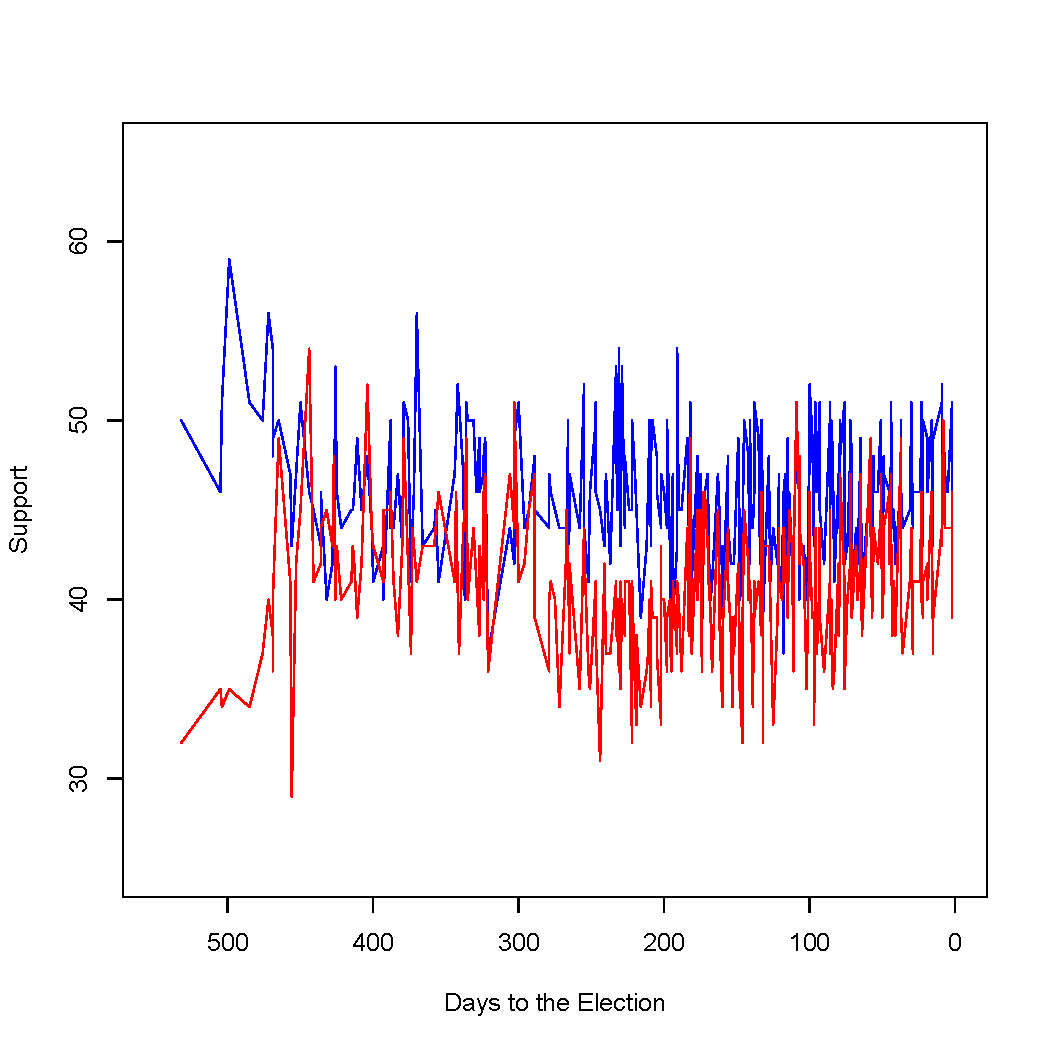
\includegraphics[width=5cm]{/Users/florianhollenbach/Documents/GitHub/Polisci209_2018/slides/week6/Pollslines.pdf}
\end{center}
\end{frame}



\begin{frame}[label={sec:orgad8ff74}]{Prediction with polls}
\begin{itemize}
\item Never trust a single poll
\item Maybe we could smoothe the polls over time?
\item Average the polls that are close to each other
\end{itemize}
\end{frame}

\begin{frame}[label={sec:org2f602fd}]{Prediction with polls}
\begin{itemize}
\item This is called a \emph{moving average}
\item Average all the polls within a certain time window
\item Window size determines amount of smoothing
\end{itemize}
\end{frame}

\begin{frame}[label={sec:orgcaeeaf9}]{Creating a Moving Average}
\begin{itemize}
\item In \emph{R}, for each day, we subset the relevant polls and compute the average
\item That's a lot of subsetting and averaging (532 days)
\item Any ideas of how to do this fast?
\end{itemize}

\pause
\alert{Loops}
\end{frame}

\begin{frame}[fragile,label={sec:org2fc0515}]{Loops in R}
 \begin{verbatim}
for (i in X) {
    expression1
    expression2
    ...
    expressionN
}
\end{verbatim}
\end{frame}


\begin{frame}[label={sec:org90581b4}]{Loops in R}
Elements of a loop:
\begin{itemize}
\item \emph{i}: counter (can use any object name other than \emph{i})
\item \emph{X}: vector containing a set of ordered values the counter takes
\item \emph{expression}: a set of expressions that will be repeatedly evaluated
\end{itemize}


\pause

\{ \}: curly braces to define the beginning and the end
\end{frame}

\begin{frame}[fragile,label={sec:orgcc6eafa}]{Loops in R}
 Simple Example:

\begin{verbatim}
for (i in c(1,2,3,4,5) {
    print(i)
}
\end{verbatim}

What does this loop do?
\end{frame}

\begin{frame}[label={sec:orgcc53ee5}]{Loops in R}
\begin{itemize}
\item Indentation is important for the readability of code (Rstudio does this automagically)
\item Test  Code without loop first by setting the counter to a specific value
\end{itemize}
\end{frame}



\begin{frame}[fragile,label={sec:org2e96250}]{Loops in R}
 Printing out an iteration number can be helpful for debugging:

\begin{verbatim}
values <- c(1, -1, 2)
results <- rep(NA, 3)
for (i in 1:3) {
    cat("iteration", i, "\n")
    results[i] <- log(values[i])
}
\end{verbatim}
\end{frame}


\begin{frame}[fragile,label={sec:org1d93136}]{Loops in R}
 Let's create a moving average:

\begin{itemize}
\item Begin by creating vector for counter \& setting window size
\end{itemize}

\begin{verbatim}
days <- 500:26
window <- 7
\end{verbatim}
\end{frame}


\begin{frame}[fragile,shrink=25,label={sec:orgede6537}]{Loops in R}
 Create empty vectors

\begin{verbatim}
Clinton.pred <- Trump.pred <- rep(NA, length(days))
\end{verbatim}
\pause


Now the loops:
\begin{verbatim}
for (i in 1:length(days)) {
    week.data <-
        subset(polls2016,
               subset = ((DaysToElection < (days[i] + window))
                   & (DaysToElection >= days[i])))
    Clinton.pred[i] <- mean(week.data$Clinton)
    Trump.pred[i] <- mean(week.data$Trump)
}
\end{verbatim}
\end{frame}

\begin{frame}[fragile,label={sec:orge005838}]{Loops in R}
 Smoothed Plot:
\begin{verbatim}
plot(days, Clinton.pred, type = "l", col = "blue",
     xlab = "Days to the Election", ylab = "Support",
     xlim = c(550, 0), ylim = c(25, 65))
lines(days, Trump.pred, col = "red")
\end{verbatim}
\end{frame}


\begin{frame}[label={sec:org451f0ba}]{Smoothed Plot:}
\begin{center}
\includegraphics[width=5cm]{/Users/florianhollenbach/Documents/GitHub/Polisci209_2018/slides/week6/Smoothed7.pdf}
\end{center}
\end{frame}



\begin{frame}[fragile,shrink=25,label={sec:org8e5753f}]{2 week Smoothing}
 \begin{verbatim}
Clinton.pred <- Trump.pred <- rep(NA, length(days))
window <- 14

\end{verbatim}
\pause


Now the loops:
\begin{verbatim}
for (i in 1:length(days)) {
    week.data <-
        subset(polls2016,
               subset = ((DaysToElection < (days[i] + window))
                   & (DaysToElection >= days[i])))
    Clinton.pred[i] <- mean(week.data$Clinton)
    Trump.pred[i] <- mean(week.data$Trump)
}
\end{verbatim}
\end{frame}

\begin{frame}[fragile,label={sec:orga15fce0}]{2 week Smoothing}
 \begin{verbatim}
plot(days, Clinton.pred, type = "l", col = "blue",
     xlab = "Days to the Election", ylab = "Support",
     xlim = c(550, 0), ylim = c(25, 65))
lines(days, Trump.pred, col = "red")
\end{verbatim}
\end{frame}


\begin{frame}[label={sec:orgfecb89b}]{Smoothed Plot:}
\begin{center}
\includegraphics[width=5cm]{/Users/florianhollenbach/Documents/GitHub/Polisci209_2018/slides/week6/Smoothed14.pdf}
\end{center}
\end{frame}


\begin{frame}[fragile,label={sec:orgabccca8}]{Smoothed Plot:}
 Let's add some explanations/legend to the plot

\begin{verbatim}
text(400, 50, "Clinton", col = "blue")
text(400, 40, "Trump", col = "red")
\end{verbatim}
\end{frame}


\begin{frame}[fragile,label={sec:orgab66f0b}]{Smoothed Plot:}
 Let's add some explanations/legend to the plot

\begin{verbatim}
text(200, 60, "party\n conventions")
abline(v = as.Date("2016-11-8") - as.Date("2016-7-28"),
       lty = "dotted", col = "blue")
abline(v = as.Date("2016-11-8") - as.Date("2016-7-21"),
       lty = "dotted", col = "red")
text(50, 30, "debates")
abline(v = as.Date("2016-11-8") - as.Date("2016-9-26"),
       lty = "dashed")
abline(v = as.Date("2016-11-8") - as.Date("2016-10-9"),
       lty = "dashed")
\end{verbatim}
\end{frame}



\begin{frame}[label={sec:org8b5664f}]{Smoothed Plot:}
\begin{center}
\includegraphics[width=5cm]{/Users/florianhollenbach/Documents/GitHub/Polisci209_2018/slides/week6/Smoothed14_text.pdf}
\end{center}
\end{frame}
\end{document}